\begin{frame}
    \begin{center}
        \Huge{Anforderungen}
    \end{center}
\end{frame}
\begin{frame}
    \frametitle{Übersicht}
    \begin{figure}[h]
        \centering
        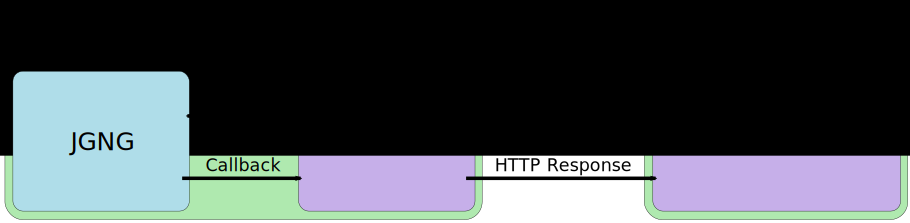
\includegraphics[width=\textwidth]{../figures/client-server.pdf}
        \caption{Übersicht Komponenten}
    \end{figure}
\end{frame}
\begin{frame}
    \frametitle{Anforderungen an die API}
    \begin{itemize}
        \item Auswahl des Algorithmus, zum Trainieren des neuronalen Netzes
        \item Einstellung aller Parameter des Algorithmus
        \item Auswahl eines Datensatzes, zum Trainieren des neuronalen Netzes
        \item Festlegung der Anzahl an Durchläufen für eine Trainingseinheit
        \item Bereitstellung der topologischen Daten des neuronalen Netzes, die der Algorithmus generiert hat
        \item Paralleles Trainieren mehrerer neuronaler Netze
    \end{itemize}
\end{frame}
\begin{frame}
    \frametitle{Anforderungen an die Webanwendung}
    \begin{itemize}
        \item Nutzung der Funktionalität der API
        \item Übersichtliche Darstellung des Trainingsprozesses des neuronalen Netzes
        \item Benutzerfreundliche Möglichkeit zur Parametrisierung des Algorithmus
    \end{itemize}
\end{frame}
